\documentclass[usenatbib,fleqn]{mnras}

\pdfoutput=1

\usepackage{amsmath}
\usepackage{amssymb}
\usepackage{blindtext}
\usepackage{bm}
\usepackage{color}
\usepackage{graphicx}
\usepackage{hyperref}
\usepackage[all]{hypcap}
% \usepackage{lineno}
\usepackage{longtable}
\usepackage{multicol}
\usepackage{multirow}
\usepackage{natbib}
% \usepackage{flushend}
\usepackage{txfonts}
\usepackage{wasysym}
\usepackage[capitalize,nameinlink]{cleveref}

% cleveref tweak to remove parentheses from equations
\creflabelformat{equation}{#2#1#3}
\crefrangelabelformat{equation}{#3#1#4 to #5#2#6}

% For links of references
\hypersetup{colorlinks,
  linkcolor=red,
  filecolor=red,
  urlcolor=magenta,
  citecolor=blue}

\usepackage{array}
\newcolumntype{L}[1]{>{\raggedright\let\newline\\\arraybackslash\hspace{0pt}}m{#1}}
\newcolumntype{C}[1]{>{\centering\let\newline\\\arraybackslash\hspace{0pt}}m{#1}}
\newcolumntype{R}[1]{>{\raggedleft\let\newline\\\arraybackslash\hspace{0pt}}m{#1}}

\newcommand{\comment}[1]{\textbf{\color{magenta} #1}}

\newcommand{\hbt}{\textsc{hbt+}}

\newcommand{\Msun}{\mathrm{M}_\odot}
\newcommand{\hMsun}{h^{-1}\,\Msun}
\newcommand{\hMpc}{h^{-1}\,\mathrm{Mpc}}
\newcommand{\subfind}{\textsc{subfind}}
\newcommand{\tcent}{t_\mathrm{cent}}
\newcommand{\tinfall}{t_\mathrm{infall}}
\newcommand{\zcent}{z_\mathrm{cent}}
\newcommand{\zinfall}{z_\mathrm{infall}}


\title[Mass content of satellites in EAGLE]{The history and mass content of cluster galaxies in the EAGLE simulation}

\author[C.\ Sif\'on]{Crist\'obal Sif\'on
\\
Department of Astrophysical Sciences, Peyton Hall, Princeton University, Princeton, NJ 08544, USA
}

% These dates will be filled out by the publisher
% \date{Accepted XXX. Received YYY; in original form ZZZ}

% Enter the current year, for the copyright statements etc.
\pubyear{2018}

\begin{document}
\label{firstpage}
\pagerange{\pageref{firstpage}--\pageref{lastpage}}

% \linenumbers

\maketitle

\begin{abstract}
%  We use the upgraded Hierarchical Bound Tree (HBT+) subhalo catalogue from the EAGLE cosmological hydrodynamical simulation to explore the effects of  of galaxies into massive ($M_{200m}>10^{13}\,\Msun$) galaxy groups and clusters.
We explore the mass content of cluster galaxies in the EAGLE cosmological hydrodynamical simulation. 
  
  We explore changes in satellite stellar mass/halo mass as a function of (the observationally accessible) distance from host/nearest cluster, as well as the more physical change as a function of time for the same satellites.
  
  We identify the progenitors of $z=0.18$ satellites as \textbf{some population of centrals at some earlier time}, and find \textbf{the following problems arise when interpreting differences between present-day satellites with present-day centrals}

\end{abstract}



\section{Wish/thought list}


\comment{are all quantities in the HBT catalogs in units of $h$, or is the value of $h$ already included?}
\\

(Given in the order they came to my head)

\begin{enumerate}
  \item Explore what difference does it make where did the satellite come from, by binning as a function of cluster-centric distance but also, for galaxies not part of the cluster, by host mass (probably do not need groups less massive than $10^{12}\,h^{-1}\,\Msun$, as that's already the mass of the Milky Way). Another way is, for galaxies not part of a massive cluster, to see how far they are to a massive cluster and what is their host mass. For a given distance to a massive cluster, does the mass relation change with host mass? We may need to control by distance from host center as well, and then it may become too noisy...
  \item try to find a good definition for subhalo size using the density profiles. Perhaps differences between our measurements and EAGLE are caused by a model error?
  \item Plot stellar-to-total mass \emph{ratios} as a function of cluster-centric distance.
  \item When plotting ``distance to nearest cluster'' as opposed to distance to \emph{host} cluster, should 
  \item Use some definition of ``phase-space distance'', similar to the bins in Fig 1 of Muzzin+14.
\end{enumerate}

\subsection{Literature notes}

\begin{enumerate}
  \item \citet{rhee17}: weak preprocessing in general ($<30\%$ mass loss prior to entering cluster). Mass lost up to 1st pericenter $\sim$20-30\%, constant with time (Fig 4)
\end{enumerate}

\subsection{New thoughts emerging from my \hbt\ exploration:}
\begin{enumerate}
  \item To see what produces changes (especially fluctuations) in mass, should look at the location of the (sub)halo and its neighbors. It's probably that their spiraling into each other or so.
\end{enumerate}



\section{Introduction}

In this paper we refer generically to ``galaxy groups'' as all galaxy associations more massive than $M_{200m}=10^{11}\,\hMsun$, and to ``clusters'' as the subset of those groups which have $M_{200m}>10^{13}\,\Msun$. (This is a more relaxed definition of ``cluster'' than usual.) Throughout, we refer to masses $M_{\Delta m}$ ($M_{\Delta c}$) as the mass containing $\Delta$ times the mean (critical) density of the Universe at the group redshift. Where appropriate, we adopt the cosmology used in the EAGLE simulations,  with \textbf{parameters...}


\section{Simulation}

Our study is based on the upgraded Hierarchical Bound Tree \citep[HBT+,][]{han18} post-processing Evolution and Assembly of Galaxies and their Environment (EAGLE) simulations \citep{schaye15,crain15}. EAGLE is a suite of cosmological hydrodynamical simulations with varying box sizes, resolutions, and baryonic feedback prescriptions. The simulation we use here is labelled \texttt{RefL0100N1504} and has a box size of $(100\,\hMpc)^3$, with N particles and mass resolutions of X,Y,Z for dark matter, gas and stars, respectively.

Haloes were identified in EAGLE using a standard friends-of-friends algorithm with a linking length of X, and subhaloes were identified using the upgraded . \cite{knebe11} found that \subfind\ tends to underpredict subhalo masses at all halo-centric distances. While uncertainties on the bias were not reported by \cite{knebe11}, the smooth behaviour of the bias as a function of halo-centric distance suggests that uncertainties are rather small, and we neglect them in our analysis. By interpolating figure 8 of \cite{knebe11}, we apply the following correction to all subhalo and galaxy masses reported in the EAGLE database:
\begin{equation}\label{eq:subfind_correction}
  \Delta m_\mathrm{sub}(x) = ...
\end{equation}
where $x=R/R_{200m}$ is the three-dimensional distance normalized by the halo size.\footnote{\cite{knebe11} reported their results in terms of $R_{200c}$ and $M_{200c}$. We convert from $R_{200c}$ to $R_{200m}$ using \textbf{a mass-concentration relation consistent with EAGLE -- look for one}.}

We adopt the location of the minimum of the gravitational potential as the position of all subhaloes, consistent with \cite{velliscig17}.

\Cref{f:massfunction} shows the mass functions of 

\begin{figure}
  \centerline{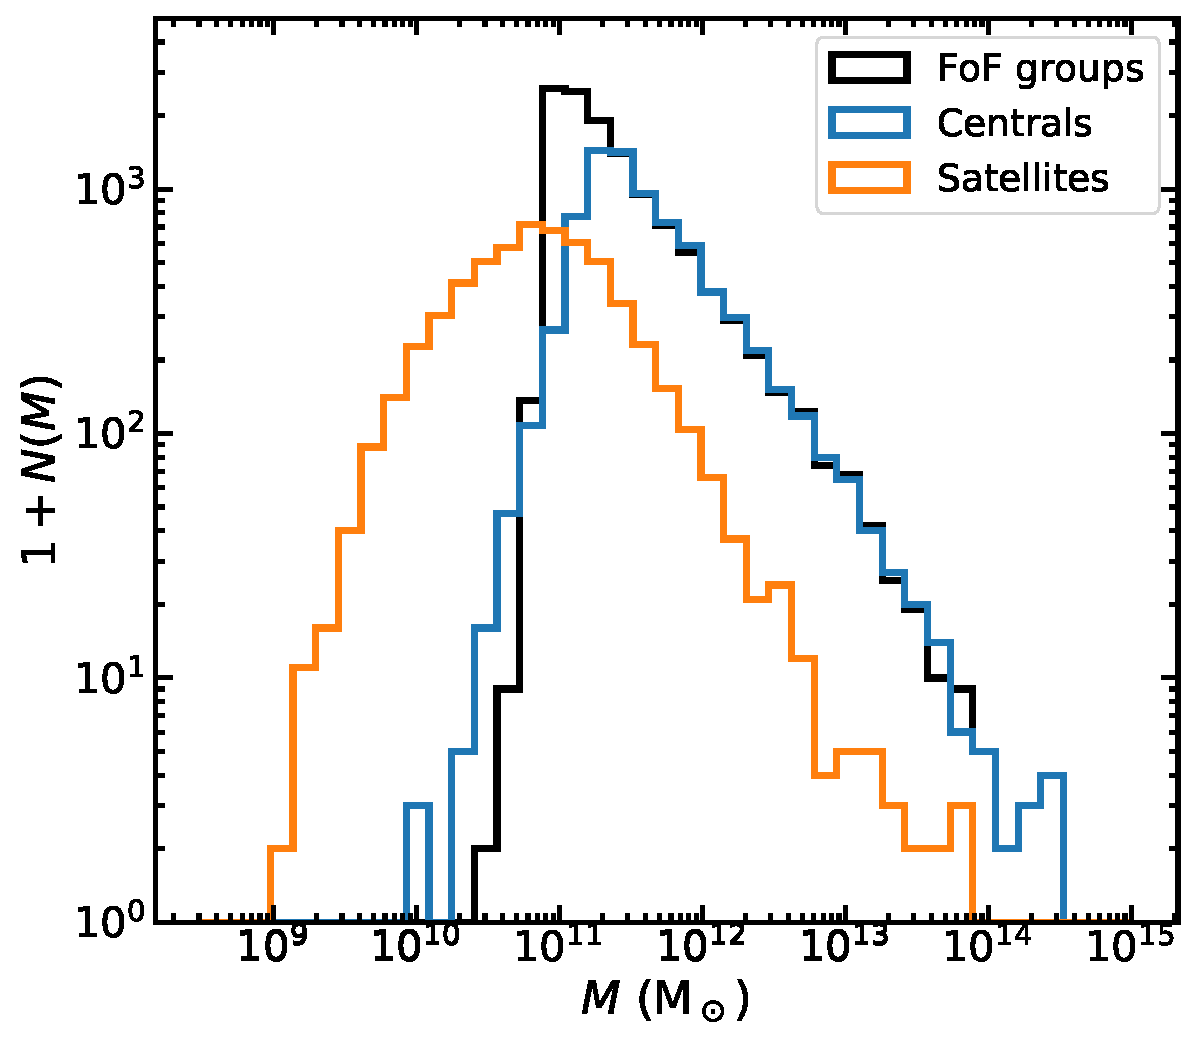
\includegraphics[width=\linewidth]{massfunction.pdf}}
\caption{Mass function of galaxy groups with $M_{200m}>10^{11}\,\hMsun$ and central and satellite galaxies in the EAGLE RefL0100N1504 simulation.}
\label{f:massfunction}
\end{figure}


\begin{figure}
  \centerline{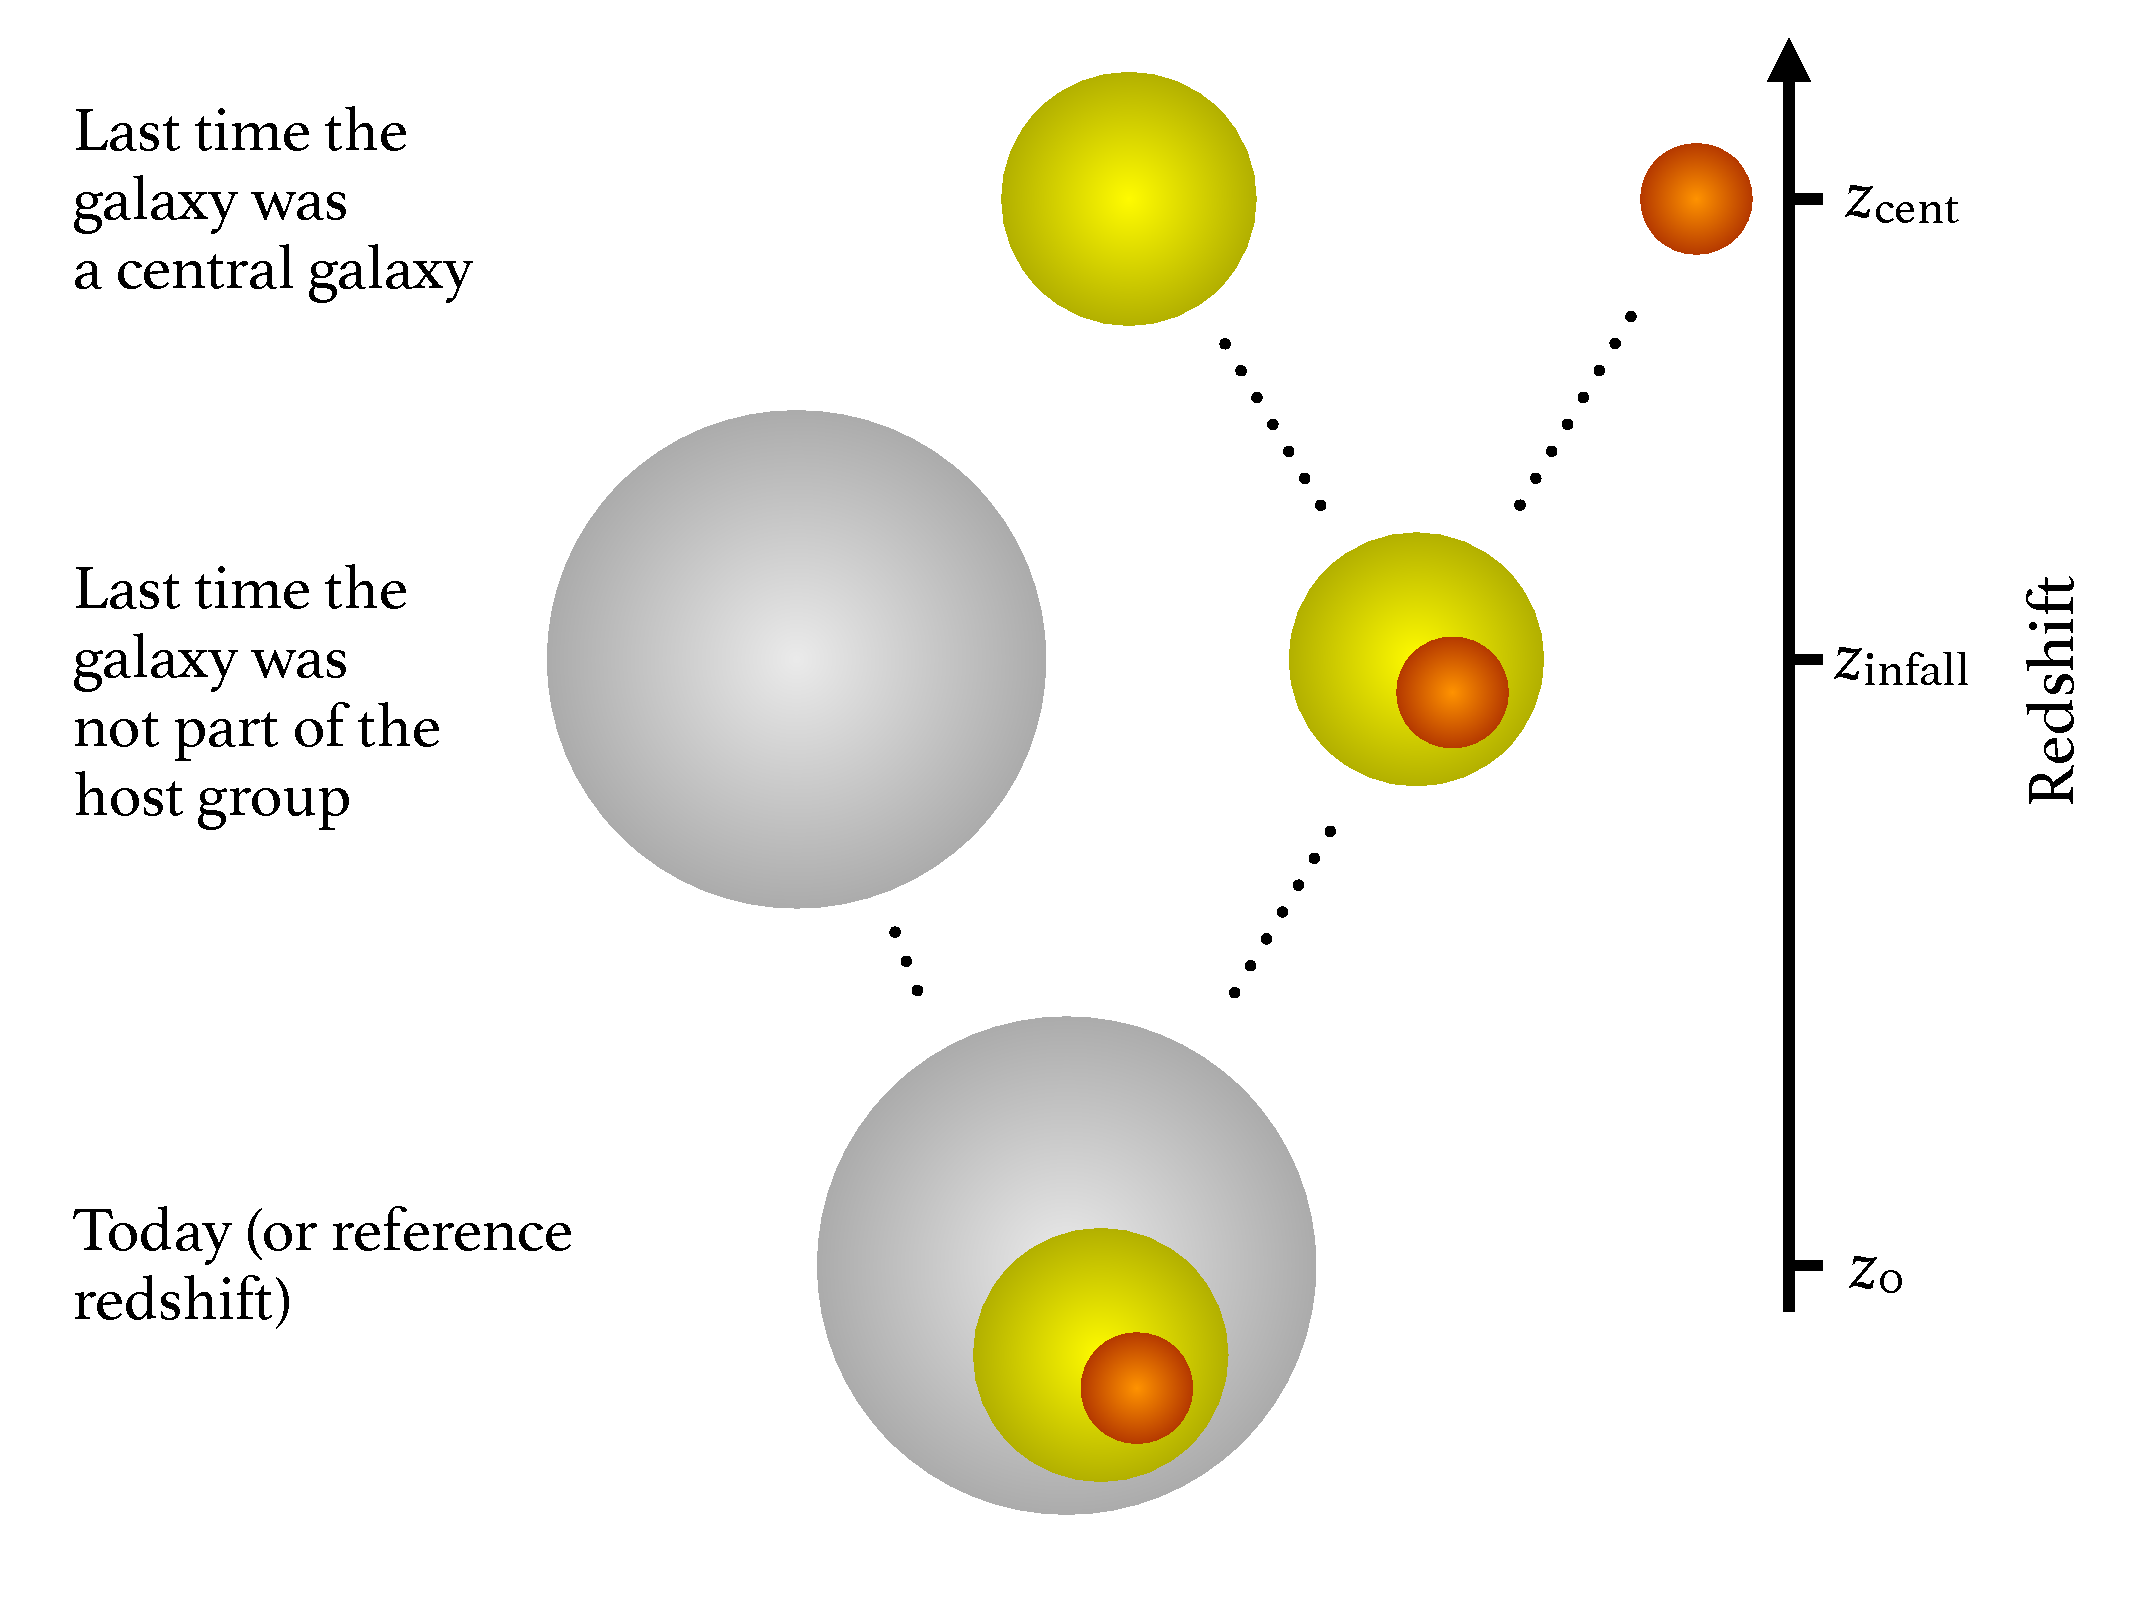
\includegraphics[width=\linewidth]{history_chart.pdf}}
\caption{Schematic figure showing the relevant times we consider in this work. The brown circle represents a galaxy of interest, which is a satellite at redshift $z_0$, part of a host group shown in grey. We identify the last redshift at which the brown satellite was hosted by the grey host as $\zinfall$. The last time at which the brown satellite was a central galaxy is labelled $\zcent$. When the brown satellite fell into the grey host (identified at present with \texttt{GroupID}), it may in fact have already been part of another group, shown in green. If this is the case, then $\zcent \neq \zinfall$.}
\label{f:history_chart}
\end{figure}

\section{The evolution of present-day subhalos}

\begin{itemize}
  \item show something like the fraction of subhalos that were centrals at infall (i.e., $\tcent = \tinfall$) as a function of halo mass, subhalo mass, and infall time.
\end{itemize}


\begin{figure*}
  \centerline{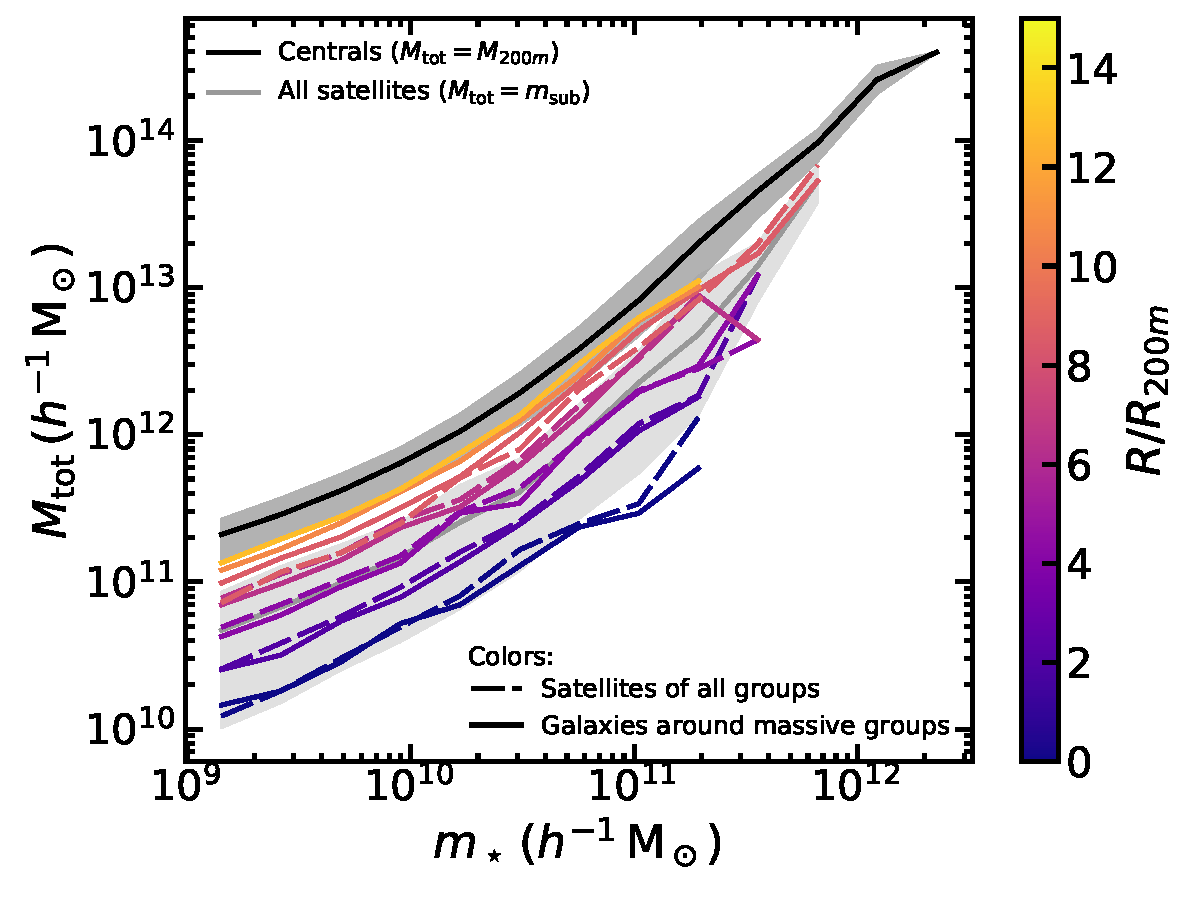
\includegraphics[width=\linewidth]{total_to_stellar_groups_and_clusters.pdf}}
\caption{The total-to-stellar mass relation of galaxies as a function of distance to their \emph{host} group (dashed lines), and as a function of their distance to the \emph{nearest} massive ($M_{200m}>10^{13}\,h^{-1}\,\Msun$) cluster (dotted lines), each normalized by the size of the group/cluster. The blue line shows the average total-to-stellar mass relation of all satellites belonging to all groups, and the black line shows the total-to-stellar mass relation of central galaxies. In the latter two, the respective shaded regions show the scatter in each.}
\label{f:relation}
\end{figure*}

\Cref{f:relation} shows that:
\begin{enumerate}
  \item the TSMR of subhaloes is approximately a factor 4 lower than that of centrals.
  \item the TSMR decreases in amplitude as we get closer to the cluster centre, but its shape does not change.
  \item If cluster size is accounted for, the TSMR of subhaloes does not depend on cluster mass (i.e., dashed and dotted lines of the same color overlap), except perhaps for low-mass galaxies outside $R_{200m}$. \emph{This suggests that massive clusters exert their influence out to larger radius compared to low-mass clusters}, especially for low-mass galaxies ($m_\mathrm{gal}\lesssim10^{-2}M_\mathrm{cl}$).
\end{enumerate}

Caveats:
\begin{enumerate}
 \item Need to check how much of point (ii) may be caused by biases in subfind (compare to the curve of recovered versus true mass as a function of radius from Knebe+11).
 \item Remove centrals of massive groups from the coloured curves.
 \item Remember that Marco showed that the satellite fraction is really off in EAGLE (compared to GAMA), so should not mix centrals and satellites, nor take the satellite fraction seriously (?).
 \item It seems like the subfind bias is pretty large and may be driving most if not all the changes we see as a function of $R$. Perhaps I could gauge this bias by comparing an EAGLE DM only sim with a DM only Rockstar catalog? Even then, baryonic effects on density profiles could conceivably change the comparison.
\end{enumerate}


\section{Application to satellite lensing measurements}


\bibliographystyle{mnras}
\bibliography{bibliography}






\end{document}


